%%%%%%%%%%%%%%%%%%%%%%%%%%%%%%%%%%%%%%%%%
% Stylish Article
% LaTeX Template
% Version 2.1 (1/10/15)
%
% This template has been downloaded from:
% http://www.LaTeXTemplates.com
%
% Original author:
% Mathias Legrand (legrand.mathias@gmail.com) 
% With extensive modifications by:
% Vel (vel@latextemplates.com)
%
% License:
% CC BY-NC-SA 3.0 (http://creativecommons.org/licenses/by-nc-sa/3.0/)
%
%%%%%%%%%%%%%%%%%%%%%%%%%%%%%%%%%%%%%%%%%

%----------------------------------------------------------------------------------------
%	PACKAGES AND OTHER DOCUMENT CONFIGURATIONS
%----------------------------------------------------------------------------------------

\documentclass[fleqn,10pt]{SelfArx} % Document font size and equations flushed left

\usepackage[english]{babel} % Specify a different language here - english by default

\usepackage{lipsum} % Required to insert dummy text. To be removed otherwise

%----------------------------------------------------------------------------------------
%	COLUMNS
%----------------------------------------------------------------------------------------

\setlength{\columnsep}{0.55cm} % Distance between the two columns of text
\setlength{\fboxrule}{0.75pt} % Width of the border around the abstract

%----------------------------------------------------------------------------------------
%	COLORS
%----------------------------------------------------------------------------------------

\definecolor{color1}{RGB}{0,0,90} % Color of the article title and sections
\definecolor{color2}{RGB}{0,20,20} % Color of the boxes behind the abstract and headings

%----------------------------------------------------------------------------------------
%	HYPERLINKS
%----------------------------------------------------------------------------------------

\usepackage{hyperref} % Required for hyperlinks
\hypersetup{hidelinks,colorlinks,breaklinks=true,urlcolor=color2,citecolor=color1,linkcolor=color1,bookmarksopen=false,pdftitle={Title},pdfauthor={Author}}

%----------------------------------------------------------------------------------------
%	ARTICLE INFORMATION
%----------------------------------------------------------------------------------------

\JournalInfo{Handout, No. 1, \today} % Journal information
\Archive{Dieses Werk ist unter einer Creative Commons Lizenz vom Typ Namensnennung 2.0 Deutschland zugänglich. Um eine Kopie dieser Lizenz einzusehen, konsultieren Sie http://creativecommons.org/licenses/by/2.0/de/ oder wenden Sie sich brieflich an Creative Commons, Postfach 1866, Mountain View, California, 94042, USA.} % Additional notes (e.g. copyright, DOI, review/research article)

\PaperTitle{12 Factor App} % Article title

\Authors{Sidney Kuyateh\textsuperscript{1}, Steffen Walter\textsuperscript{2}} % Authors
\affiliation{\textsuperscript{1}\textit{Studiengang Informationstechnik, Fakultät Technik, Duale Schule Baden-Württemberg, Stuttgart}} % Author affiliation
\affiliation{\textsuperscript{2}\textit{Studiengang Informationstechnik, Fakultät Technik, Duale Schule Baden-Württemberg, Stuttgart}} % Author affiliation
\affiliation{*\textbf{Corresponding author}: inf17001@lehre.dhbw-stuttgart.de} % Corresponding author

\Keywords{} % Keywords - if you don't want any simply remove all the text between the curly brackets
\newcommand{\keywordname}{Keywords} % Defines the keywords heading name

%----------------------------------------------------------------------------------------
%	ABSTRACT
%----------------------------------------------------------------------------------------

\Abstract{Das vorliegende Handout soll einen kurzen Überblick über die Kriterien geben, welche bei der Erstellung einer Web-Applikation unter den Vorgaben der "12 Factor App" beachtet werden müssen.\newline Mit der "12 Factor App" hat Adam Wiggins von der Firma Heroku im Jahr 2011 eine Methode vorgestellt, mit der sich Software-As-A-Service (SaaS) Apps entwerfen und umsetzten lassen, die folgenden Kriterien entsprechen:
\begin{itemize}
	\item Deklarative Formate zur Kosten- und Zeitoptimierung
	\item Klare Schnittstellen zum Betriebssystem für maximale Portabilität
	\item Deploymentmöglichkeiten für modernen Cloudplattformen
	\item Minimierung des Wegs von der Entwicklung zum produktiven Einsatz, für maximale Agilität
	\item Die Möglichkeit zur einfachen Skalierung, ohne weitreichende Änderungen
\end{itemize}}

%----------------------------------------------------------------------------------------

\begin{document}

\flushbottom % Makes all text pages the same height

\maketitle % Print the title and abstract box

%\tableofcontents % Print the contents section

\thispagestyle{empty} % Removes page numbering from the first page

%----------------------------------------------------------------------------------------
%	ARTICLE CONTENTS
%----------------------------------------------------------------------------------------

\section*{Einleitung} % The \section*{} command stops section numbering

\addcontentsline{toc}{section}{Introduction} % Adds this section to the table of contents
Die Entwickler der 12 Factor App stammen von der Firma Heroku, wo sie der Entwicklung Zahlreicher Webapplikationen im Bereich SaaS beigewohnt haben, um dann die Synthese ihrer Erfahrungen in einem Dokument zu Sammeln und zu Veröffentlichen.\newline
Das Ziel dabei ist es, dass SaaS Apps künftig einfacher skalierbar sind, besser durch ein Team gepflegt und auf Dauer mit kalkulierbaren Kosten weiterentwickelt werden können. Das Konzept richtet sich gleichermaßen an Entwickler wie auch an Administratoren, die mit dem Deployment betraut sind.

%------------------------------------------------

\section{Die Zwölf Faktoren}
\subsection{I. Codebase}
\subsection{II. Abhängigkeiten}
\subsection{III. Konfiguration}
\subsection{IV. Unterstützende Dienste}
\subsection{V. Build, Release, Run}
\subsection{VI. Prozesse}
%Sidney
\subsection{VII. Bindung an Ports}
\subsection{VIII. Nebenläufigkeit}
\subsection{IX. Entsorgbarkeit}
\subsection{X. Dev-Prod-Gleichheit}
\subsection{XI. Logs}
\subsection{XII.\@ Administrationsprozesse}
\section{Fazit}

\begin{figure}[ht]\centering % Using \begin{figure*} makes the figure take up the entire width of the page
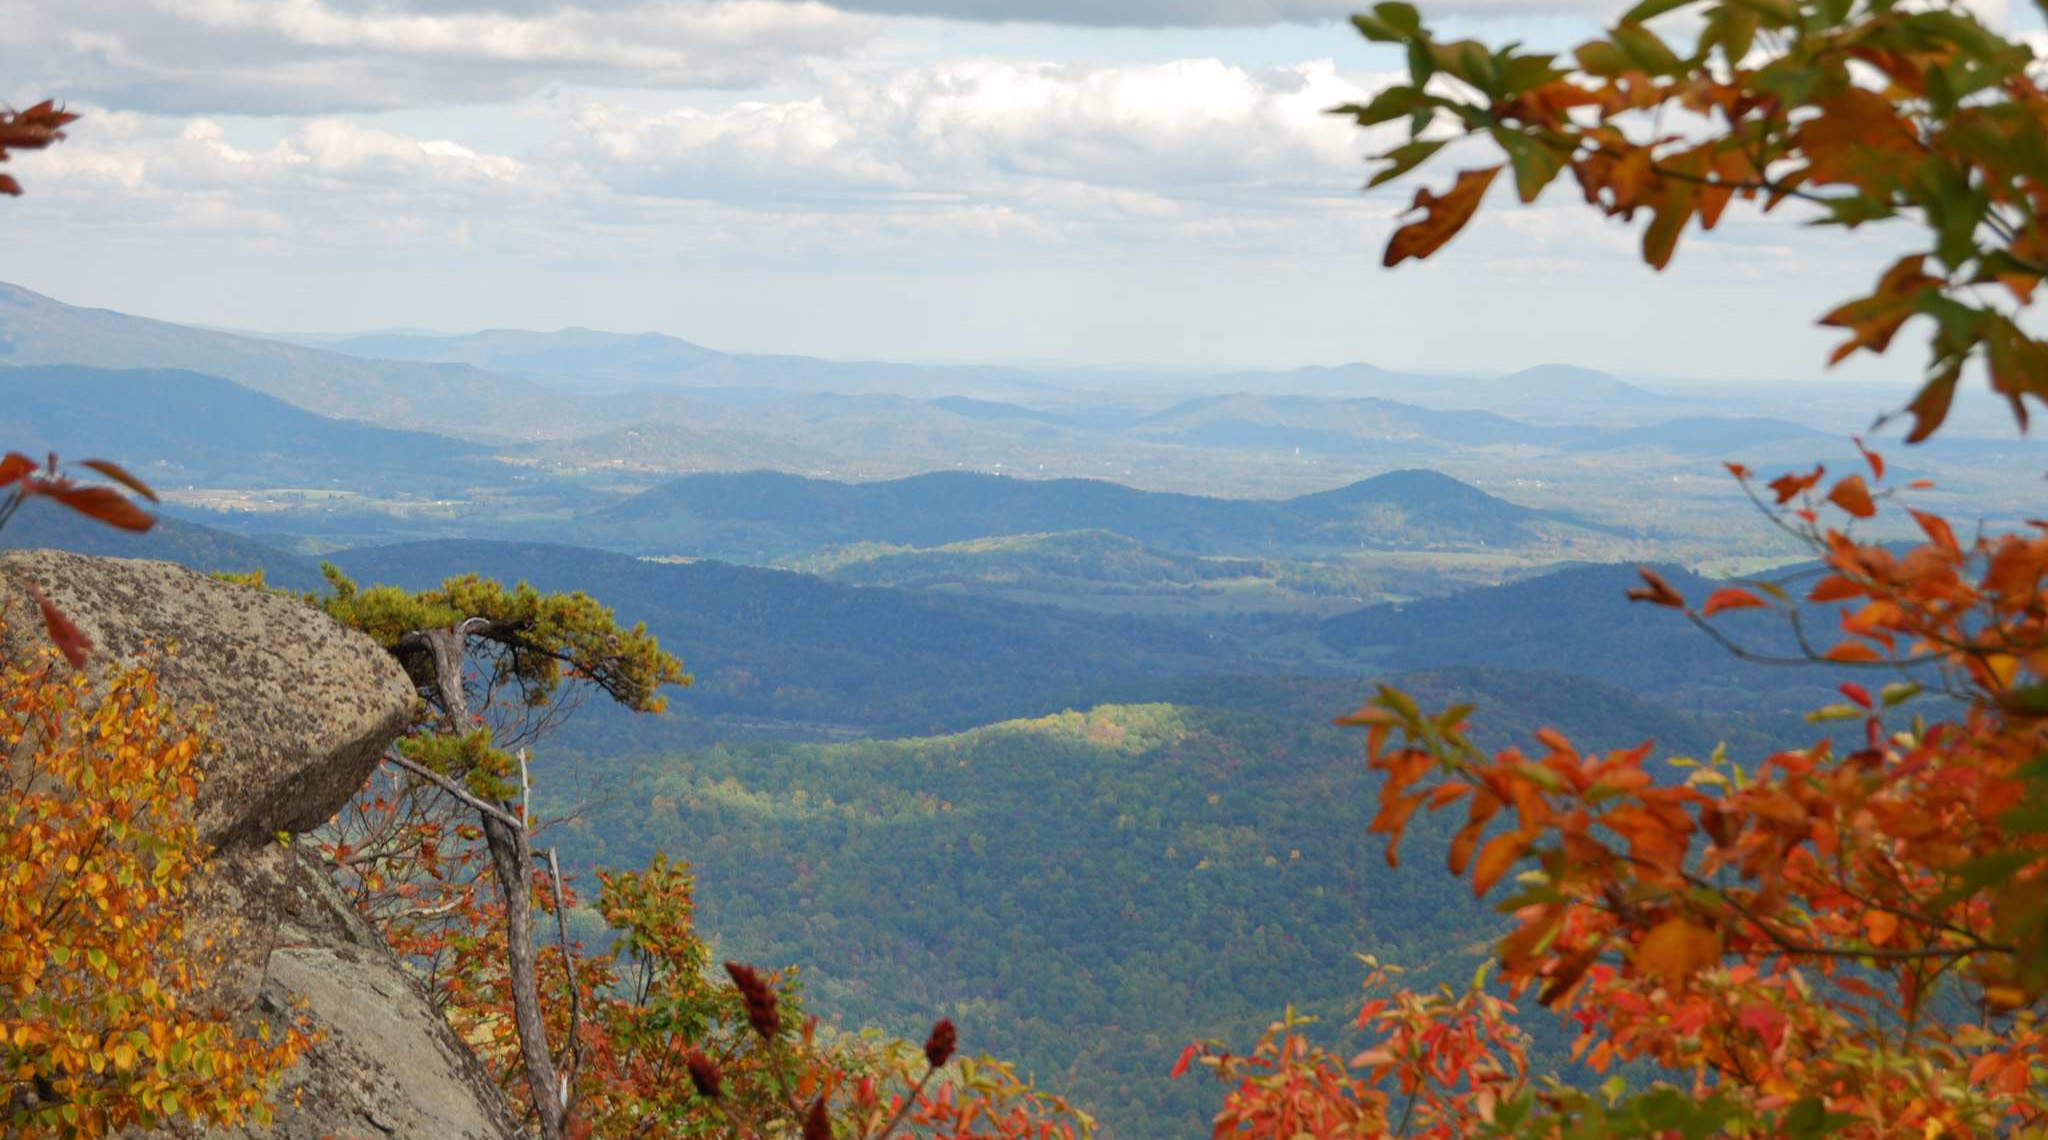
\includegraphics[width=\linewidth]{view}
\caption{Wide Picture}
\label{fig:view}
\end{figure*}

\lipsum[4] % Dummy text


%------------------------------------------------


\addcontentsline{toc}{section}{Acknowledgments} % Adds this section to the table of contents

So long and thanks for all the fish \cite{Figueredo:2009dg}.

%----------------------------------------------------------------------------------------
%	REFERENCE LIST
%----------------------------------------------------------------------------------------
\phantomsection
\bibliographystyle{unsrt}
\bibliography{sample}

%----------------------------------------------------------------------------------------

\end{document}